% Chapter Template

\chapter{Ensayos y resultados} % Main chapter title
En este capítulo se detallan los ensayos realizados en trenes en conjunto con el personal de SOFSE. En las secciones que siguen se explican las mediciones realizadas en las visitas a los talleres de Victoria y Castelar de Trenes Argentinos Operaciones. Se presenta el detalle de las mediciones, un análisis de datos de las tramas obtenidas, detalle del hardware de las placas de control de los carteles de matriz led, y se presentan algunas pruebas de integración necesarias para validar el desarrollo. \\


\label{Chapter4} % Change X to a consecutive number; for referencing this chapter elsewhere, use \ref{ChapterX}

%----------------------------------------------------------------------------------------
%	SECTION 1
%----------------------------------------------------------------------------------------

\section{Primeras mediciones sobre la red de comunicaciones}

Uno de los objetivos generales del proyecto en el que se enmarcó este trabajo, era relevar las soluciones existentes de la red TCN y PIDS. A lo largo del desarrollo, se realizaron reuniones de trabajo con el personal de Trenes Argentinos Operaciones, y visitas a los talleres de la Gerencia de Material Rodante Eléctrico,  para relevar información técnica del sistema de comunicaciones del tren. En orden cronológico, incluyendo trabajo realizado en etapa de confinamiento por COVID-19, se resaltan algunas de las siguientes interacciones con SOFSE:\\


\begin{enumerate}

\item 2020-05-20: se ensayaron mediciones sobre la maqueta de los talleres de Castelar, coordinadas de forma remota, para obtener mediciones de datos de la red RS485 del sistema PIDS.

\item 2020-06-30: se ensayaron mediciones sobre formaciones ferroviarias operativas en los talleres de Victoria, relevando los puntos de interconexión de la red TCN con el TLCD (pantalla táctil del conductor). Se realizaron también mediciones en el punto de interconexión del bus MVB con el módulo RCMe. 

\item 2020-09-23: se ensayaron nuevas mediciones, coordinadas de forma remota, en la maqueta de Castelar con un nuevo módulo analizador de datos.

\item 2021-04-09: se relevaron los puntos de interconexión entre RCMe y el PIDS, y entre los módulos IDU y SCU en formaciones operativas en los talleres de Victoria. También se ensayaron mediciones sobre el bus de datos RS485 que conecta el SCU con la DACU.

\item 2021-06-04: se ensambló una maqueta local usando un cartel led compatible con la serie de los carteles de trenes relevados y se presentó como informe de avance.

\end{enumerate}


En la figura \ref{fig:maquetaCastelar} se muestra la maqueta instalada en los talleres de Castelar. Se puede observar un rack con los módulos del sistema PIDS, incluyendo la pantalla LCD táctil que maneja el conductor. También se observan los carteles de matriz led frontal (cartel grande), de salón (cartel chico) y el mapa led con el recorrido de las estaciones (cartel del medio).\\
 
\begin{figure}[H]
	\centering
	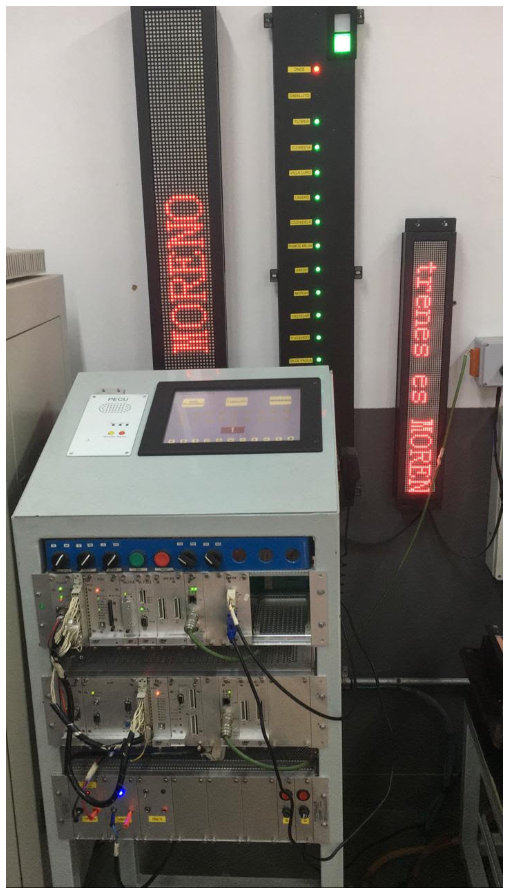
\includegraphics[width=0.66\textwidth]{./Figures/maqueta.png}
	\caption{Maqueta en talleres de Castelar.}
	\label{fig:maquetaCastelar}
\end{figure}


Durante las visitas a los talleres de Victoria, se pudo acceder a los planos eléctricos del sistema de comunicaciones del tren, correspondientes a la versión de TCN instalada en las formaciones. Esta información resultó muy relevante, ya que permitió comprender la lógica de interconexión de los módulos de hardware del tren y preparar un sistema de medición. La documentación disponible al momento de realizar los ensayos, presentaba detalles de la comunicación entre el módulo TCMS y PIDS. Esta comunicación es bidireccional y sigue un esquema \textit{Master-Slave}, donde el TCMS (Master) envía una trama y el PIDS (Slave) responde con otra. La información disponible de las tramas se detalla con el diagrama de la figura \ref{fig:tramasHeaderPayload}

\begin{figure}[H]
	\centering
	\includegraphics[width=1\textwidth]{./Figures/tramasHeaderPayload.png}
	\includegraphics[width=1\textwidth]{./Figures/tramasBitsIDU.png}
	\caption{Contenido de las tramas de datos entre TCMS y PIDS.}
	\label{fig:tramasHeaderPayload}
\end{figure}

Se puede observar que para las tramas del \textit{Master} y del \textit{Slave}, los encabezados (HEADER) y final de trama (EOF) son distintos entre sí, la carga útil (PAYLOAD) reserva 20 y 32 bytes repespectivamente, y por lo tanto la trama que responde el PIDS es de mayor longitud que la que envía TCMS. La información de los módulos IDU está contenida en los bits 0-1 de los bytes 20-28 de la trama respuesta del PIDS. Se ha resaltado en color los bits que corresponden a los módulos IDU, y se puede observar según la nomenclatura, que existen hasta 18 unidades de estos módulos, agrupados de a pares por cada salón. \\


\section{Análisis de mediciones}

Para realizar mediciones entre la red TCN y el PIDS, hizo falta encontrar la interconexión. El punto de medición está entre el módulo TCMS y la PCU, referido al diagrama de la red PIDS de la introducción, y se detalla en el esquema de la figura \ref{fig:TCMS-PIDS}. Se puede observar el bus de datos compuesto por las líneas RS485: 4001, 4002 y 4005.\\

\begin{figure}[H]
	\centering
	\includegraphics[width=0.33\textwidth]{./Figures/TCMS-PIDS.png}
	\caption{Diagrama esquemático del punto de medición entre TCMS y PIDS.}
	\label{fig:TCMS-PIDS}
\end{figure}

Para medir este punto, hizo falta intervenir el cableado con un analizador lógico para obtener tramas de datos. En el análisis de estas tramas, se pudo verificar la consistencia de la comunicación \textit{Master-Slave}, y en particular los encabezados y finales de trama. En la figura \ref{fig:tramasHeaderPayload} se presenta una captura del archivo de mediciones, evaluada con el analizador lógico programable, donde se observan los valores  0xCC y 0xC6 para el encabezado y final de tramas tipo Master, y 0xC2 y 0xC6 respectivamente para Slave. \\

\begin{figure}[H]
	\centering
	\includegraphics[width=0.75\textwidth]{./Figures/TCMS-PIDS-data.png}
	\caption{Captura del análisis de datos donde se verifican encabezados y finales de trama.}
	\label{fig:TCMS-PIDS-Data}
\end{figure}

Los parámetros de configuración utilizados para el análisis son:

\begin{itemize}
\item Baud rate: 19200 bps.
\item Data bits: 8.
\item Check digit 1 odd parity.
\item Starting position: 1.
\item Stop position: 1.
\end{itemize}

Si bien este análisis presenta consistencia con la documentación, no era suficiente para obtener la información de cómo se envían los datos al cartel de matriz led. \\

\section{Mediciones sobre la interconexión con los carteles}

En las sucesivas visitas a las instalaciones de Trenes Argentinos, se pudo estudiar en detalle los componentes internos del sistema PIDS. Hemos visto que los carteles de matriz led se encuentran distruibuidos por todos los coches de los trenes, y que se conectan a redes RS485, que son el estándar que siguen las redes del sistema PIDS y de la TCN. Este tipo de redes es muy utilizada para transmisión y recepción de datos, ya que tiene interfaces eléctricas muy robustas que usan señales diferenciales, y que normalmente se implementan en cables de par trenzado, permitiendo cableados extensos con buena inmunidad al ruido eléctrico.  \\

En la figura \ref{fig:conexionOriginal} se presenta un diagrama esquemático del punto de medición SCU-IDU, que es donde se conectan los carteles de matriz led, seguido de una fotografía de la unidad de rack donde se encuentra esta interconexión. La conexión original muestra un grupo de tres cables nomenclados como 4330a, 4330b y 4330s, correspondientes a las líneas RS485a, RS485b y RS485c respectivamente, que son las líneas que llegan a la placa de control del cartel de matriz led (IDU). Como se puede observar en la fotografía, estas líneas en conjunto con otras son cables negros que terminan en un mismo conector Harting de 48 pines. Por lo tanto, había que resolver una manera de intervenir esta interconexión a la hora de realizar mediciones.\\

\begin{figure}[H]
	\centering
      \includegraphics[width=0.25\textwidth]{./Figures/conexionOriginal.png}
      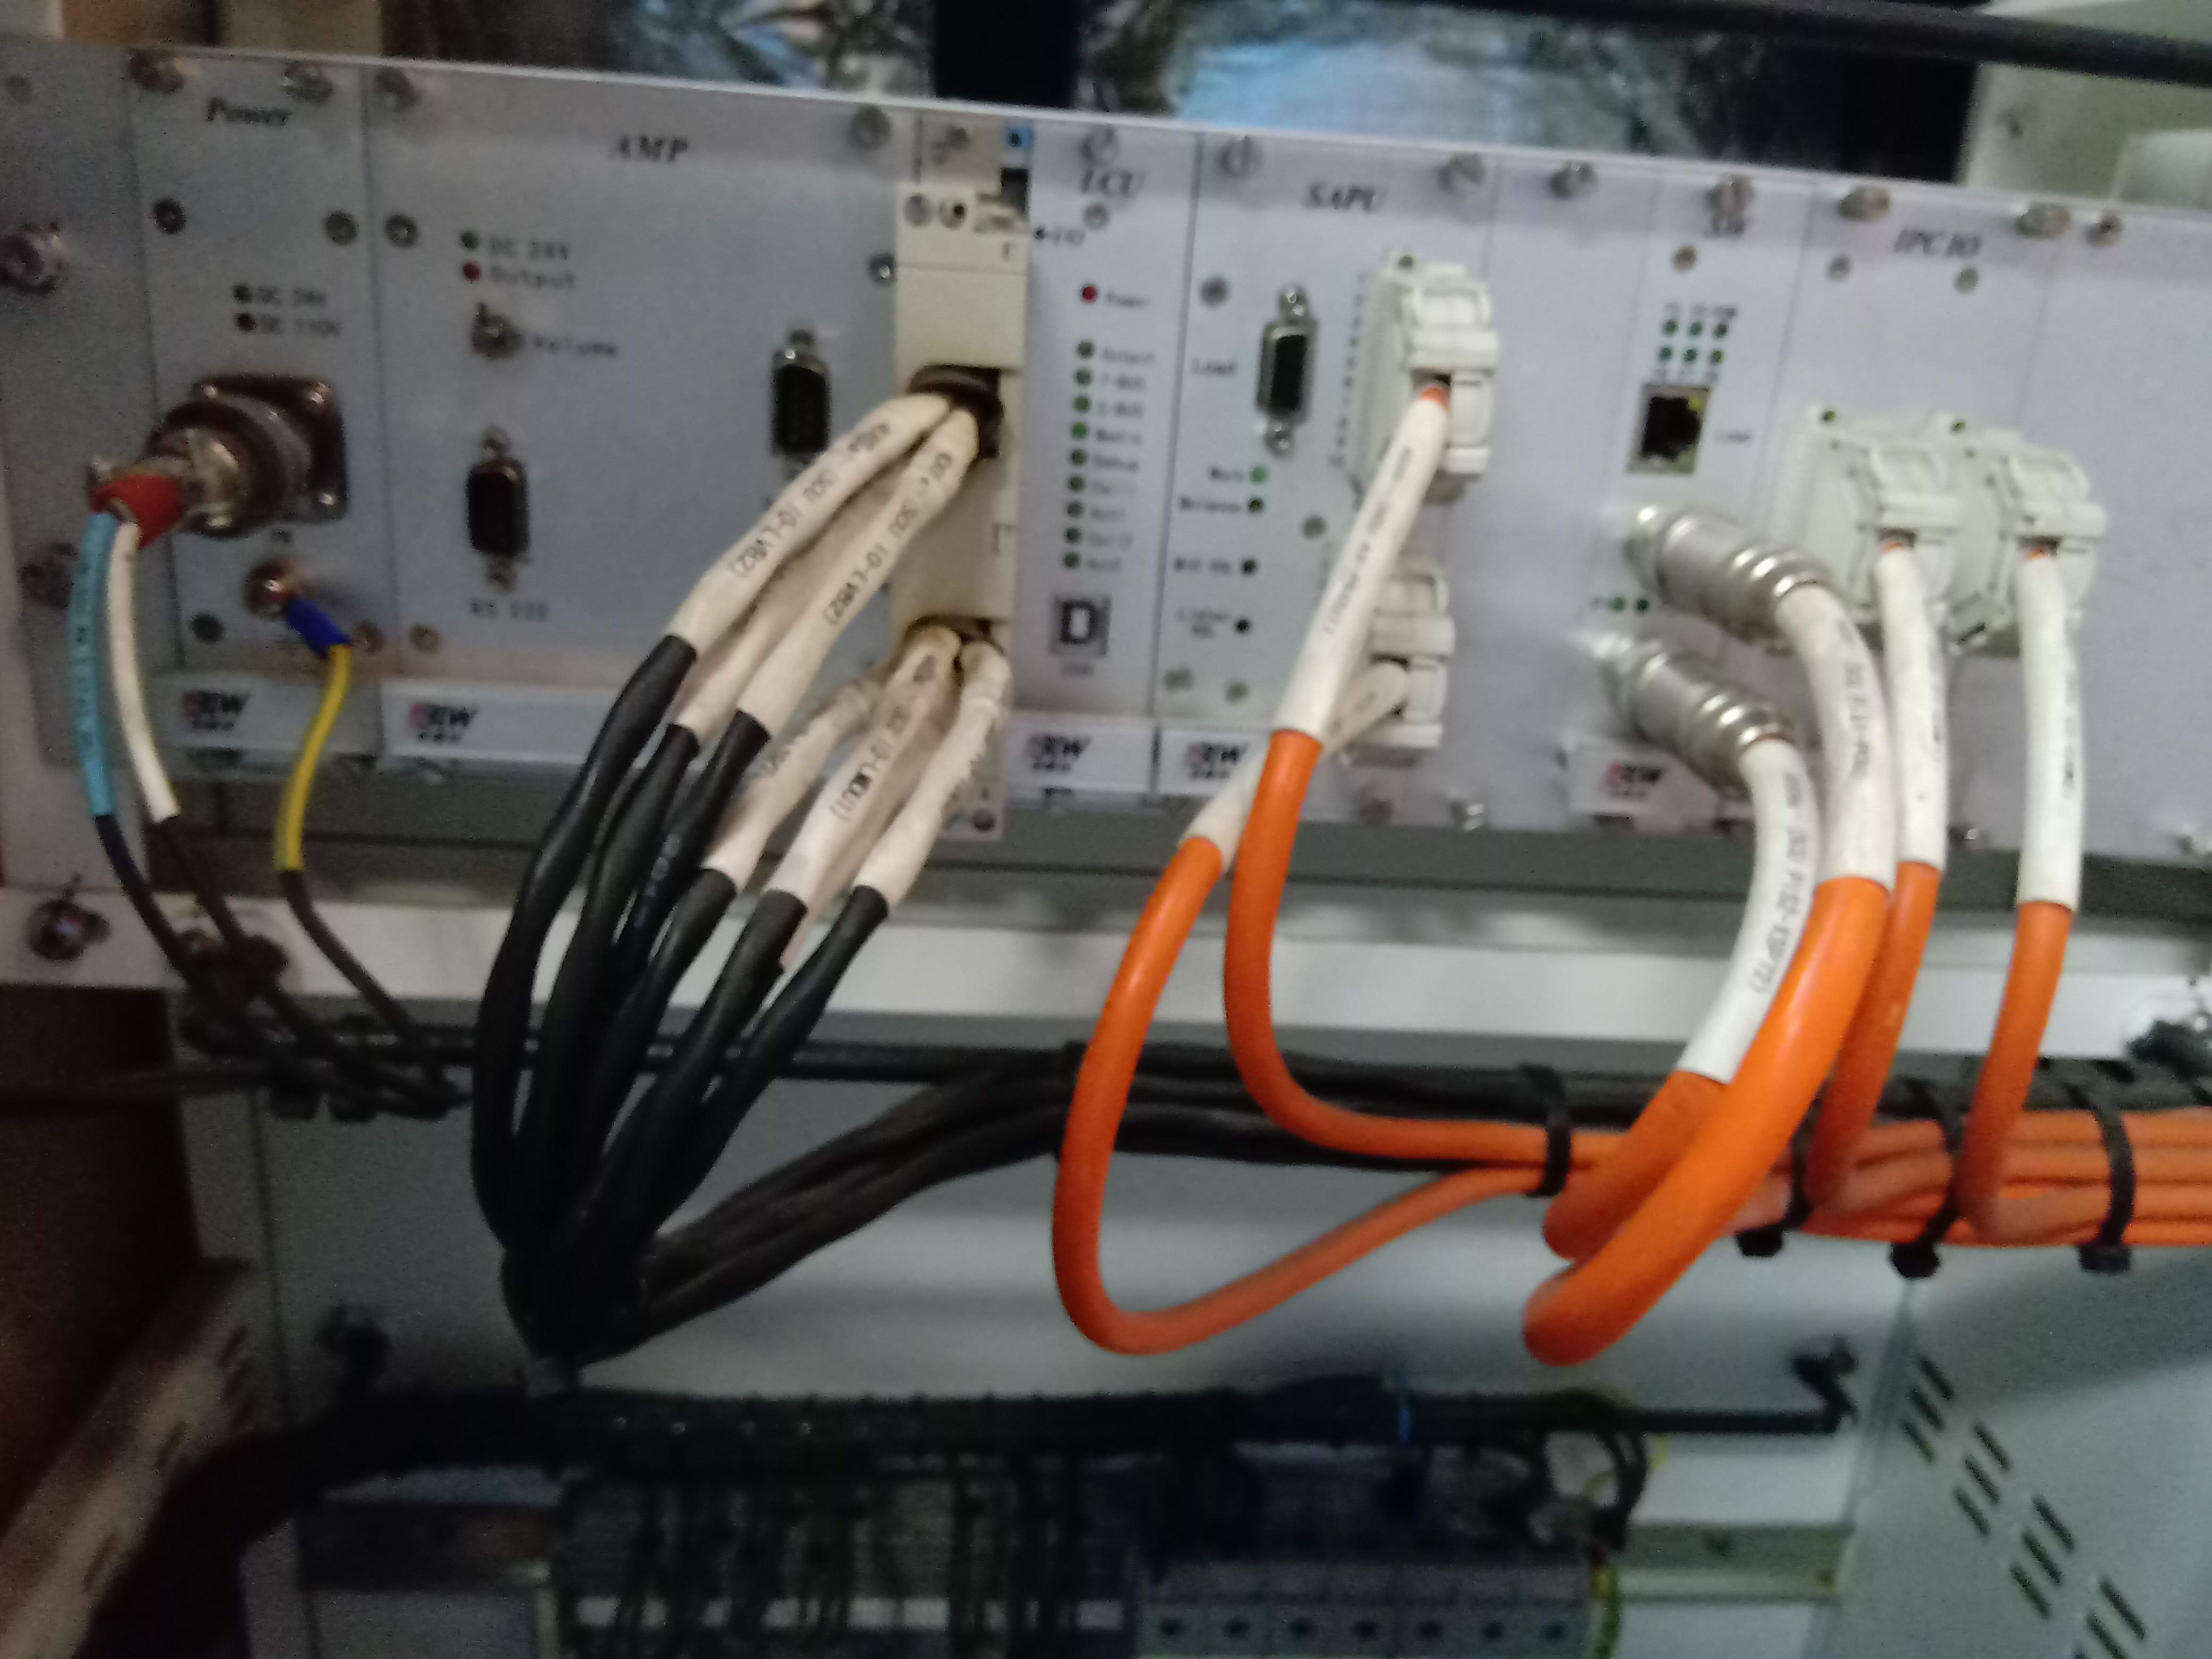
\includegraphics[width=0.5\textwidth]{./Figures/rackPIDS2.jpg}
	\caption{Diagrama esquemático y fotografía del punto de medición en la conexión SCU-IDU.}
	\label{fig:conexionOriginal}
\end{figure}


Como consecuencia de las visitas, se desarrollaron componentes para realizar mediciones in-situ, a partir del relevamiento de estos conectores y conexiones entre módulos. En la figura \ref{fig:sniffer} se muestra una fotografía del kit desarrollado para realizar mediciones en vivo en los trenes. El dispositivo cuenta con conectores de entrada y salida Harting de 48 pines, y funciona como capturador, conversor y analizador de paquetes de red para las líneas de red RS485 que corresponden al IDU, al SCU y al PCU. Este dispositivo permitió conectarse al punto de interconexión IDU-SCU mientras operaba en vivo.\\


\begin{figure}[H]
	\centering
	\includegraphics[width=0.66\textwidth]{./Figures/sniffer.jpg}
	\caption{Pieza de hardware desarrollada ad-hoc para realizar mediciones.}
	\label{fig:sniffer}
\end{figure}

 La conexión intervenida se muestra con un diagrama esquemático en la figura fig. \ref{fig:conexionIntervenida}. Por un lado está el camino original, y por el punto de corte aparece un bloque en punteado que contiene un conversor RS485 a Protocolo Serie y un analizador lógico programable, para transmitir los datos en vivo por puerto USB hacia una computadora.\\

\begin{figure}[H]
	\centering
      \includegraphics[width=0.66\textwidth]{./Figures/conexionIntervenida.png}
	\caption{Diagrama esquemático y fotografía de la intervención para realizar mediciones en vivo en la conexión SCU-IDU.}
	\label{fig:conexionIntervenida}
\end{figure}

En el ensayo que se realizaron estas mediciones, también se obtuvieron datos de otros puntos, como la interconexión SCU-LDMU, y SCU. En la figura \ref{fig:mediciones} se puede apreciar el dispositivo desarrollando midiendo el punto de interconexión SCU-IDU. \\

 \begin{figure}[H]
	\centering
	\includegraphics[width=0.5\textwidth]{./Figures/mediciones.jpg}
	\caption{Foto del banco de prueba midiendo en vivo en los talleres de Victoria.}
	\label{fig:mediciones}
\end{figure}

En la figura \ref{fig:logFile} se muestra una captura de los datos obtenidos en las mediciones SCU-IDU. Las mediciones obtenidas fueron analizados y presentaron diferencias con las registradas previamente.\\

\begin{figure}[H]
	\centering
	\includegraphics[width=0.66\textwidth]{./Figures/logFile.png}
	\caption{Detalle de mediciones registradas en formato hexadecimal.}
	\label{fig:logFile}
\end{figure}

Por empezar, no estaban presentes los encabezados y finales de trama 0xCC, 0xC6, 0xC2 y 0xCE vistos para TCMS. Con un breve preprocesamiento, que primero encontró la mayor cantidad de repeticiones con los códigos 0x7E, se buscó determinar las secuencias más repetidas en las tramas medidas. Se obtuvo como ejemplo las siguientes tramas:

\begin{itemize}
\item 7EDFFFFFDEEFBFFFBFF7E
\item 7EBDFFFF7FFFFFFFFFFFFFFF39F7E
\item 7EBDFFFF7FFFFFFFFFFFFFFF39F7E
\item 7EBDFFFF7FFFFFFFFFFFFFFF39F7E
\item 7EFFFF7FFFFFFFFFFFFFEFFFA317E
\item 7E19ABF5FFFFFFFFFFFFFFFFFF7F72A85AF7E
\item 7E7CB12914AEDFFFFFFFEFFEFFBFFFFFF7F7FFFFFFFFFDFFFFB77E
\end{itemize}

Se pudo observar nuevamente que la longitud de las tramas es variable y que a priori el encabezado y final de trama parecen ser 7E. Estas observaciones extraídas del archivo de mediciones, son compatibles con información provista por el personal de SOFSE. El detalle disponible es el siguiente:

\begin{itemize}
\item 7E es comienzo y fin de trama.
\item  3° byte es con quien se quiere comunicar. 
\item  5° byte quien habla (hipótesis).
\item  SCU tiene direcciones referidas a los coches, como 13, 23, 33, 73, 83 y 93. En la línea Sarmiento se agregarían 3 coches más (43, 53 y 63).
\end{itemize}

La información de las direcciones de los carteles frontales no quedó clara con estos ensayos. Las direcciones de la DACU y PCU, que son bloques interconectados a los SCU, parecen también seguir un patrón:

\begin{itemize}
\item Los SCU terminan en 3.
\item Las DACU terminan en 2 (DACU TC1 es 12 y DACU TC2 es 22).
\item Los PCU terminan en 1 (PCU TC1 es 11 y PCU TC2 es 21).
\end{itemize}

Según la topología de la red PIDS vista, los buses de datos siguen un esquema de tres cables por bus, nomenclados como RS485-A, RS485-B y RS485-C. En particular, la conexión entre el módulo SCU y los carteles de matriz led es por medio del bloque IDU, con los cables 4330a, 4330b y 4330c, números que corresponden al cableado físico. La conexión del SCU al IDU está incluída en un conector Harting de 48 pines, donde se unen varios buses o cableados RS485 de tres líneas.  \\

\section{Hardware de control para carteles de matriz led}

Los carteles de salón están embebidos en un gabinete de metal, donde se aloja la placa de control y parte del cableado, como se puede observar en la figura \ref{fig:displayController}.

\begin{figure}[H]
	\centering
	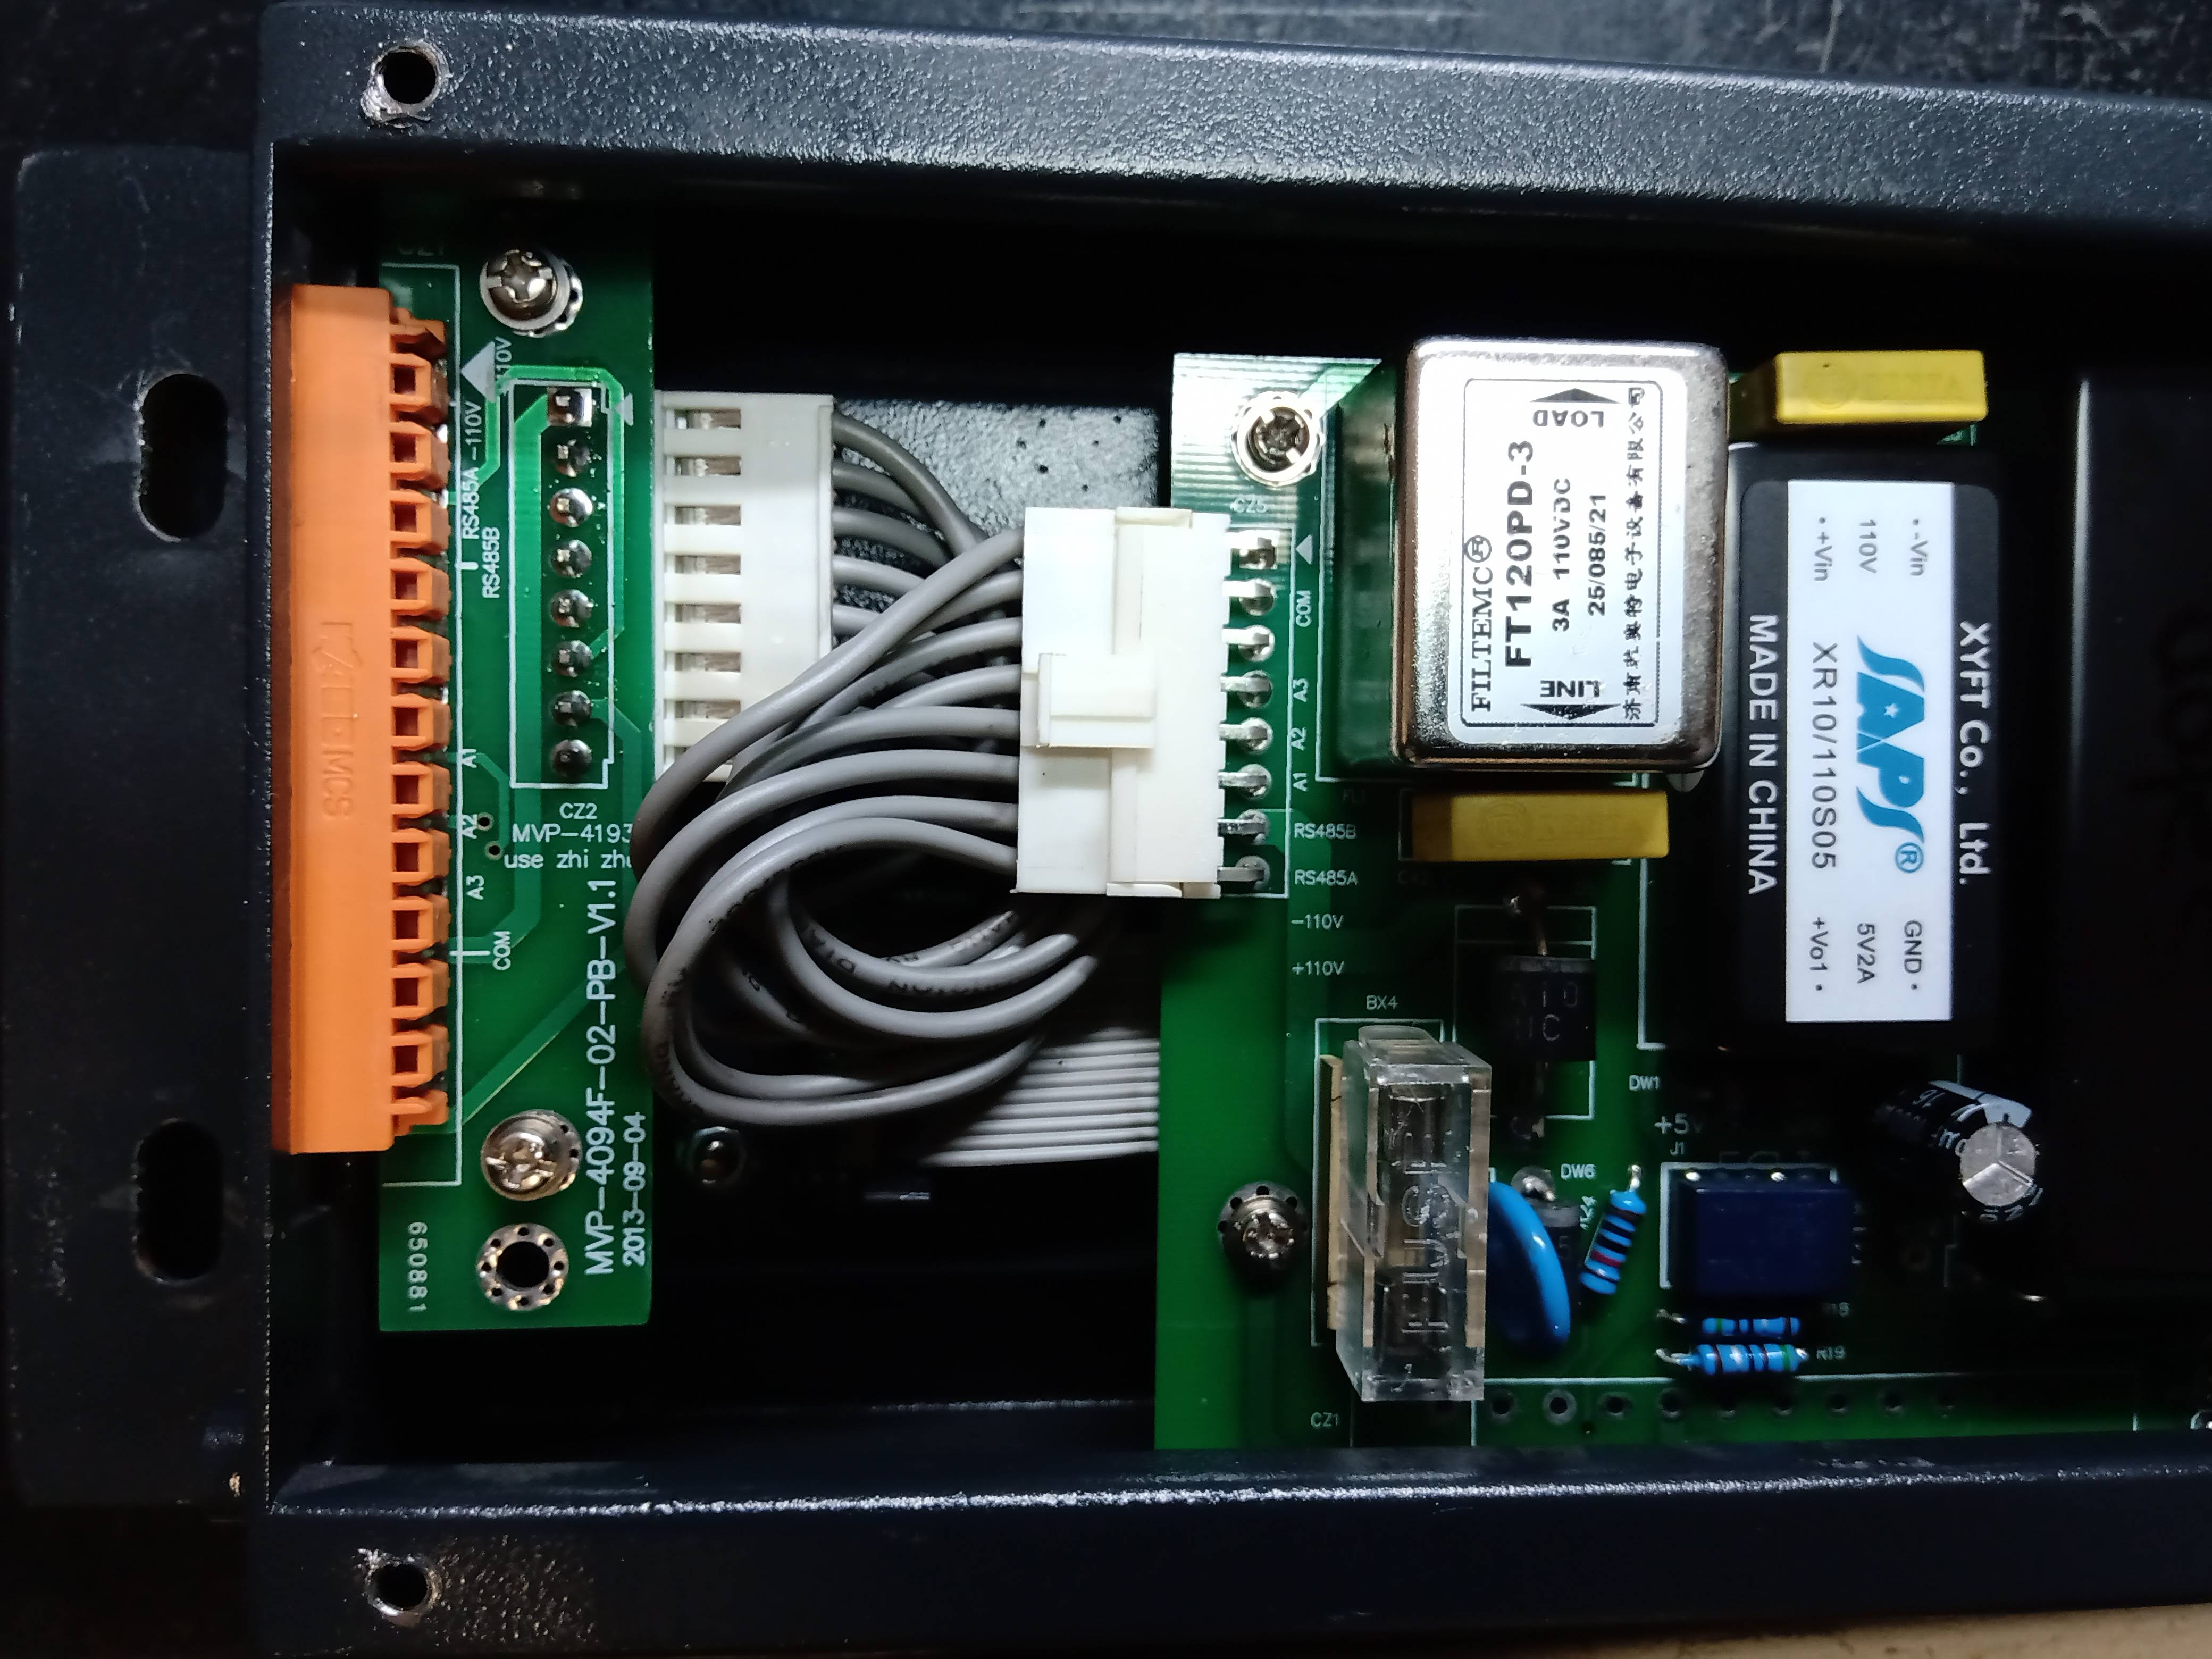
\includegraphics[width=0.6\textwidth]{./Figures/displayController.jpg}
	\caption{Fotografía del detalle de conexión de la placa de control de los carteles led de salón.}
	\label{fig:displayController}
\end{figure}

La figura \ref{fig:placa} muestra una fotografía del hardware de control de los carteles de matriz led de Trenes Argentinos.\\

\begin{figure}[H]
	\centering
	\includegraphics[width=1\textwidth]{./Figures/placaIDU.png}
	\caption{Placa de control (IDU) de los carteles de matriz led.}
	\label{fig:placa}
\end{figure}

Esta placa fue revisada en detalle y se han relevado los siguientes bloques de control:
\begin{itemize}
\item (a): Módulos de conversión de tensión.
\item (b): Circuito de optoacopladores para las señales de datos.
\item (c): Microcontrolados y circuito lógico, con conector de programación.
\item (d): Conector de entrada del bus RS485.
\item (e): Conector de salida para el cartel de matriz led.
\end{itemize}

El circuito eléctrico completo de esta placa ha sido relevado y se puede encontrar en el apéndice. Su función principal es la de decodificar las señales del tren y transmitir los mensajes al cartel de matriz led. El bloque de conversión de tensión contiene varios módulos, que son fuentes conmutadas para transformar la tensión de línea del tren de 110 Volt de corriente contínua en tensiones compatibles con el circuito de datos, por ejemplo 5 Volt o 3,3 Volt.\\


\begin{figure}[H]
	\centering
	\includegraphics[width=1\textwidth]{./Figures/cartelSOFSE.jpeg}
	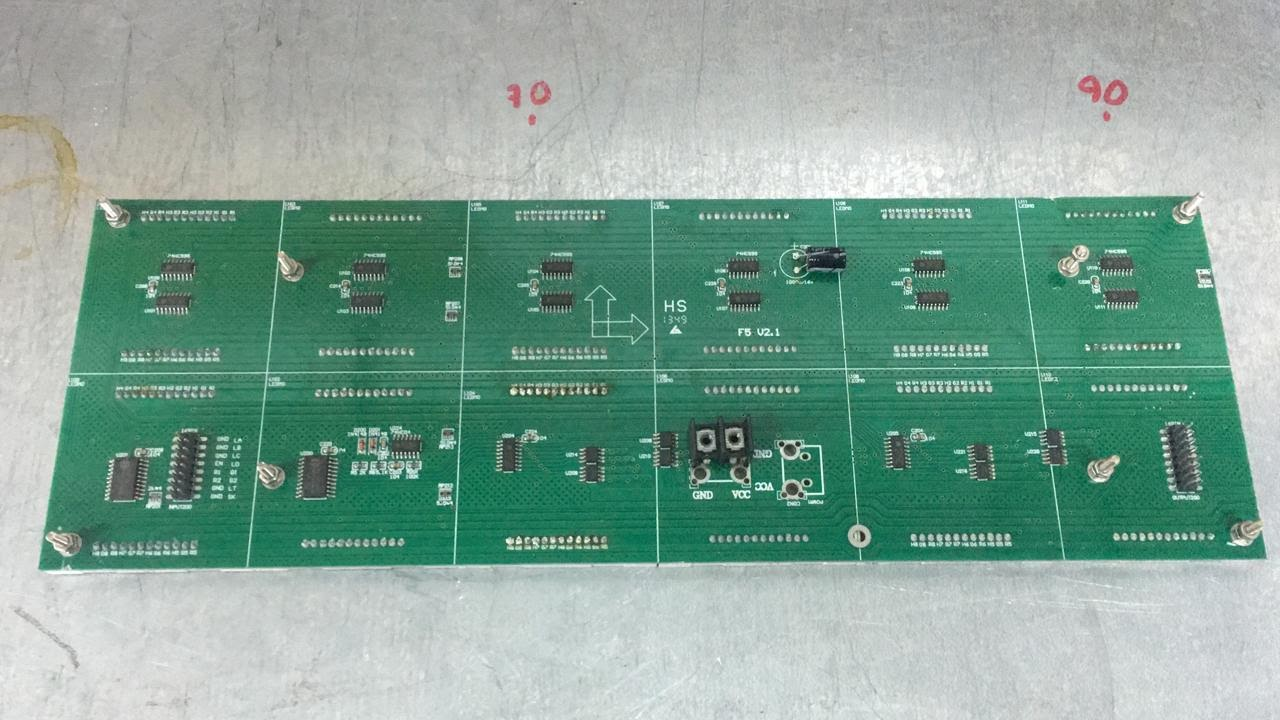
\includegraphics[width=1\textwidth]{./Figures/cartel2x6.jpeg}
	\caption{Placa de los carteles de matriz led. Arriba: frente; abajo: reverso.}
	\label{fig:placaDisplay}
\end{figure}


\begin{figure}[H]
	\centering
	\includegraphics[width=1\textwidth]{./Figures/sistema.png}
	\caption{Sistema.}
	\label{fig:sistema}
\end{figure}


\begin{figure}[H]
	\centering
	\includegraphics[width=1\textwidth]{./Figures/cartelledON.jpg}\\
	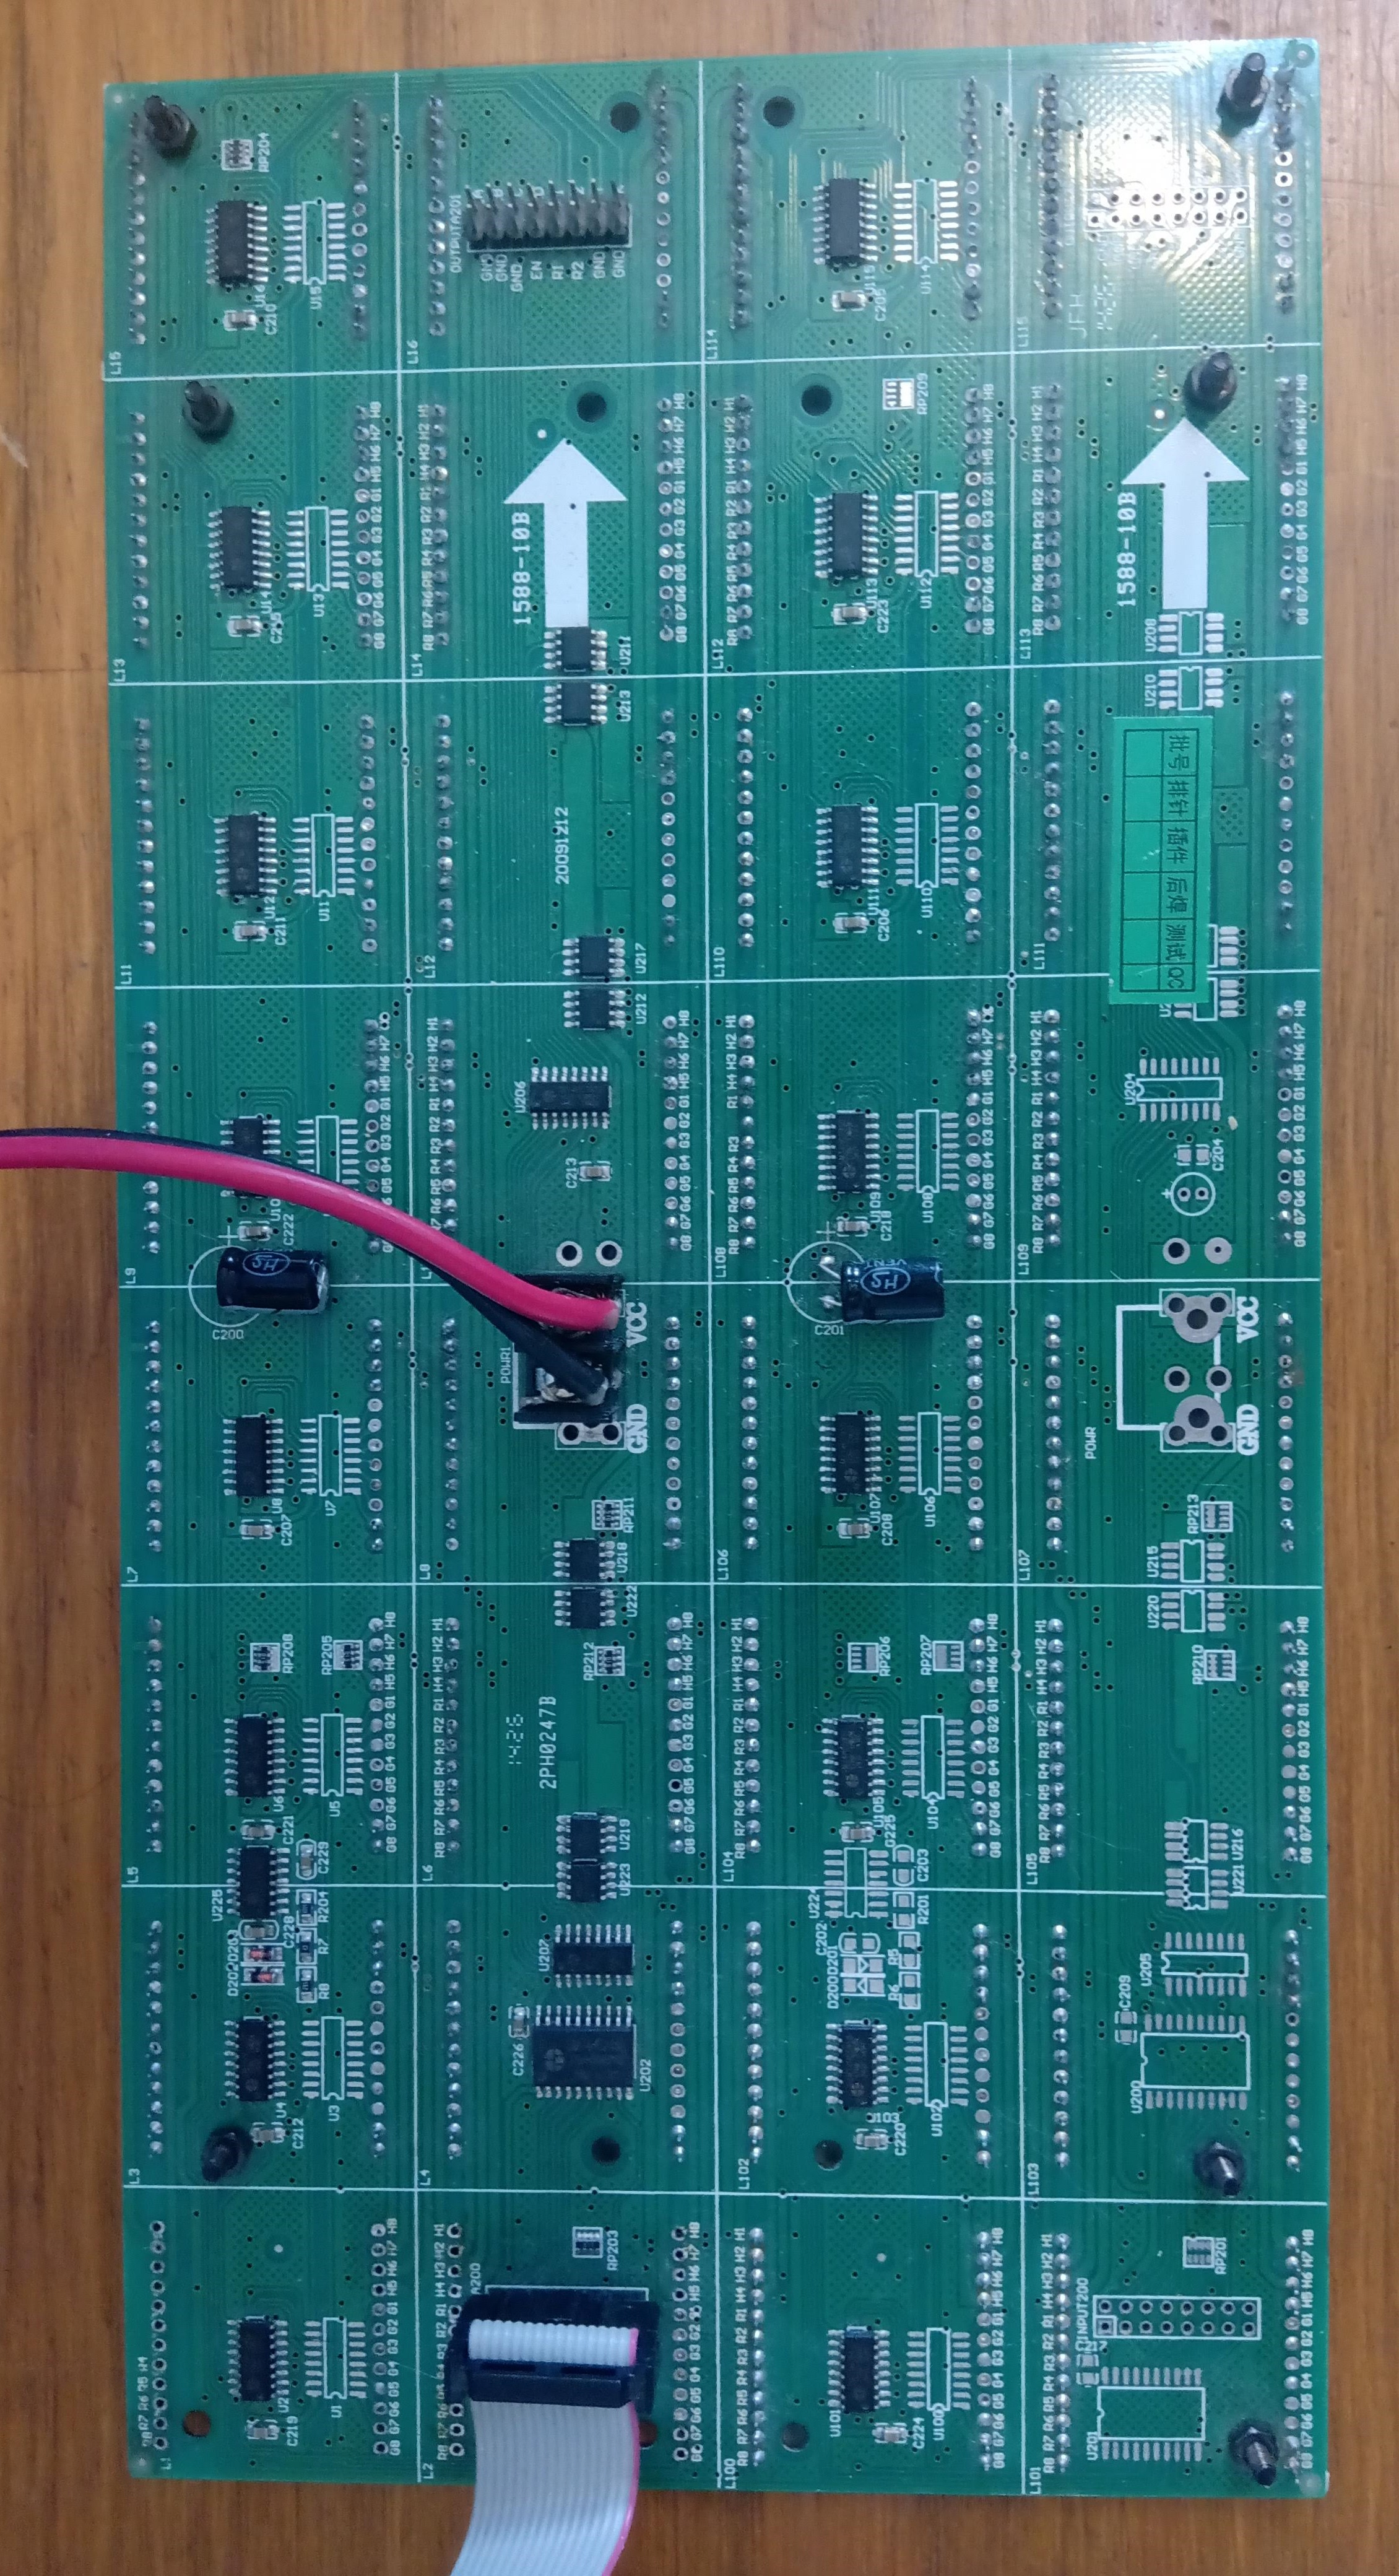
\includegraphics[width=0.75\textwidth, angle=270]{./Figures/cartel4x8.jpg}\\
	\caption{Fotografías de placas de control de los carteles de matriz led: (a) placa de 2x6 módulos; (b) placa de 4x8 módulos; (c) vista posterior de la placa de 4x8.}
	\label{fig:picsDriverled}
\end{figure}


\begin{figure}[H]
	\centering
	\includegraphics[width=1\textwidth]{./Figures/medicionesVictoria2.png}
	\caption{Fotos de la jornada de mediciones en los talleres de Victoria.}
	\label{fig:medicionesVictoria2}
\end{figure}

En la figura \ref{fig:mediciones} se muestra una fotografía del banco de medición operando en vivo en una de las formaciones ferroviaras operativas en los talleres de Victoria. Se puede observar la pieza de hardware desarrollada conectada al SCU de un lado, y a la laptop del otro. En la pantalla de la computadora se observan las líneas de datos capturadas por el analizador lógico programable.\\
En la figura \ref{fig:medicionesVictoria2} a la izquierda se puede observar la ubicación del rack de salón detrás de los asientos de pasajeros, donde están instalados los equipos de hardware de la red TCN y PIDS, y a la derecha el cartel de matriz led que está en el otro extremo de la interconexión ensayada.\\

En el circuito esquemático de la figura \ref{fig:schDriverled} se presenta el detalle de conexiones eléctricas entre bloques. Se puede observar que a la salida del conector de datos (CONN 2x8) hay dos buffers de la serie 74HC245D que direccionan las señales eléctricas a izquierda y derecha del arreglo de matrices led. A izquierda viajan las señales SER(data), SRCLK (Clock) y XXX (latch) al arreglo de Shift Registers de la serie 74HC595. Por la derecha se maneja la habilitación secuencial de las filas a través de un arreglo de decodificadores 3x8 de la serie 74HC138. Cada salida de los decodificadores se conecta a un driver de corriente en arreglo de transistores MOSFET FDS4953. Estos decodificadores cableados adecuadamente permiten manejar las 32 señales de un cartel de 4x8 módulos led. \\